% ============================================================================
\section{Preliminaries}
\label{sec:preliminaries}
% ============================================================================

Let $G$ be a (not necessarily simple) \emph{topological graph}, that is, $G$ is a graph drawn on the plane, so that the vertices of $G$ are distinct points in the plane, its edges are Jordan courves joining the corresponding pairs of points, and:%
%
\begin{inparaenum}[(i)]
\item no edge passes through a vertex different from its endpoints, 
\item no edge crosses itself and 
\item no two edges meet tangentially.
\end{inparaenum}
Let $\Gamma(G)$ be such a drawing of $G$.

An edge $e$ in $\Gamma(G)$ is called a \emph{topological edge} (or simply edge, if this is clear in the context). Edge $e$ is called \emph{true-planar}, if it is not crossed by any other edge in $\Gamma(G)$. The set of all true-planar edges of $\Gamma(G)$ forms the so-called \emph{true-planar skeleton} of $\Gamma(G)$, which we denote by $\Pi(G)$. Since $G$ is not necessarily simple, we will further assume that $\Gamma(G)$ contains neither \emph{homotopic parallel edges} nor \emph{homotopic self-loops}, that is, both the bounded and the unbounded regions defined by any self-loop or by any pair of parallel edges contain at least one vertex in their interiors. For a possitive integer $s$, a cycle of length $s$ is called \emph{true-planar $s$-cycle} if it consists of true-planar edges of $\Gamma(G)$. Let $\mathcal{F}_s=\{v_1,v_2,\ldots,v_s\}$ be a facial $s$-cycle of $\Pi(G)$ with length $s \geq 3$.  The order of the vertices (and subsequently the order of the edges) of $\mathcal{F}_s$ is determined by a walk around the boundary of $\mathcal{F}_s$ in clockwise direction. Since $\mathcal{F}_s$ is not necessarily simple, a vertex (or an edge, respectively) may appear more than once in this order; see Figure~\ref{fig:non_simple_face}.

\begin{figure}[tb]
    \centering	
	\begin{minipage}[b]{.18\textwidth}
        \centering
        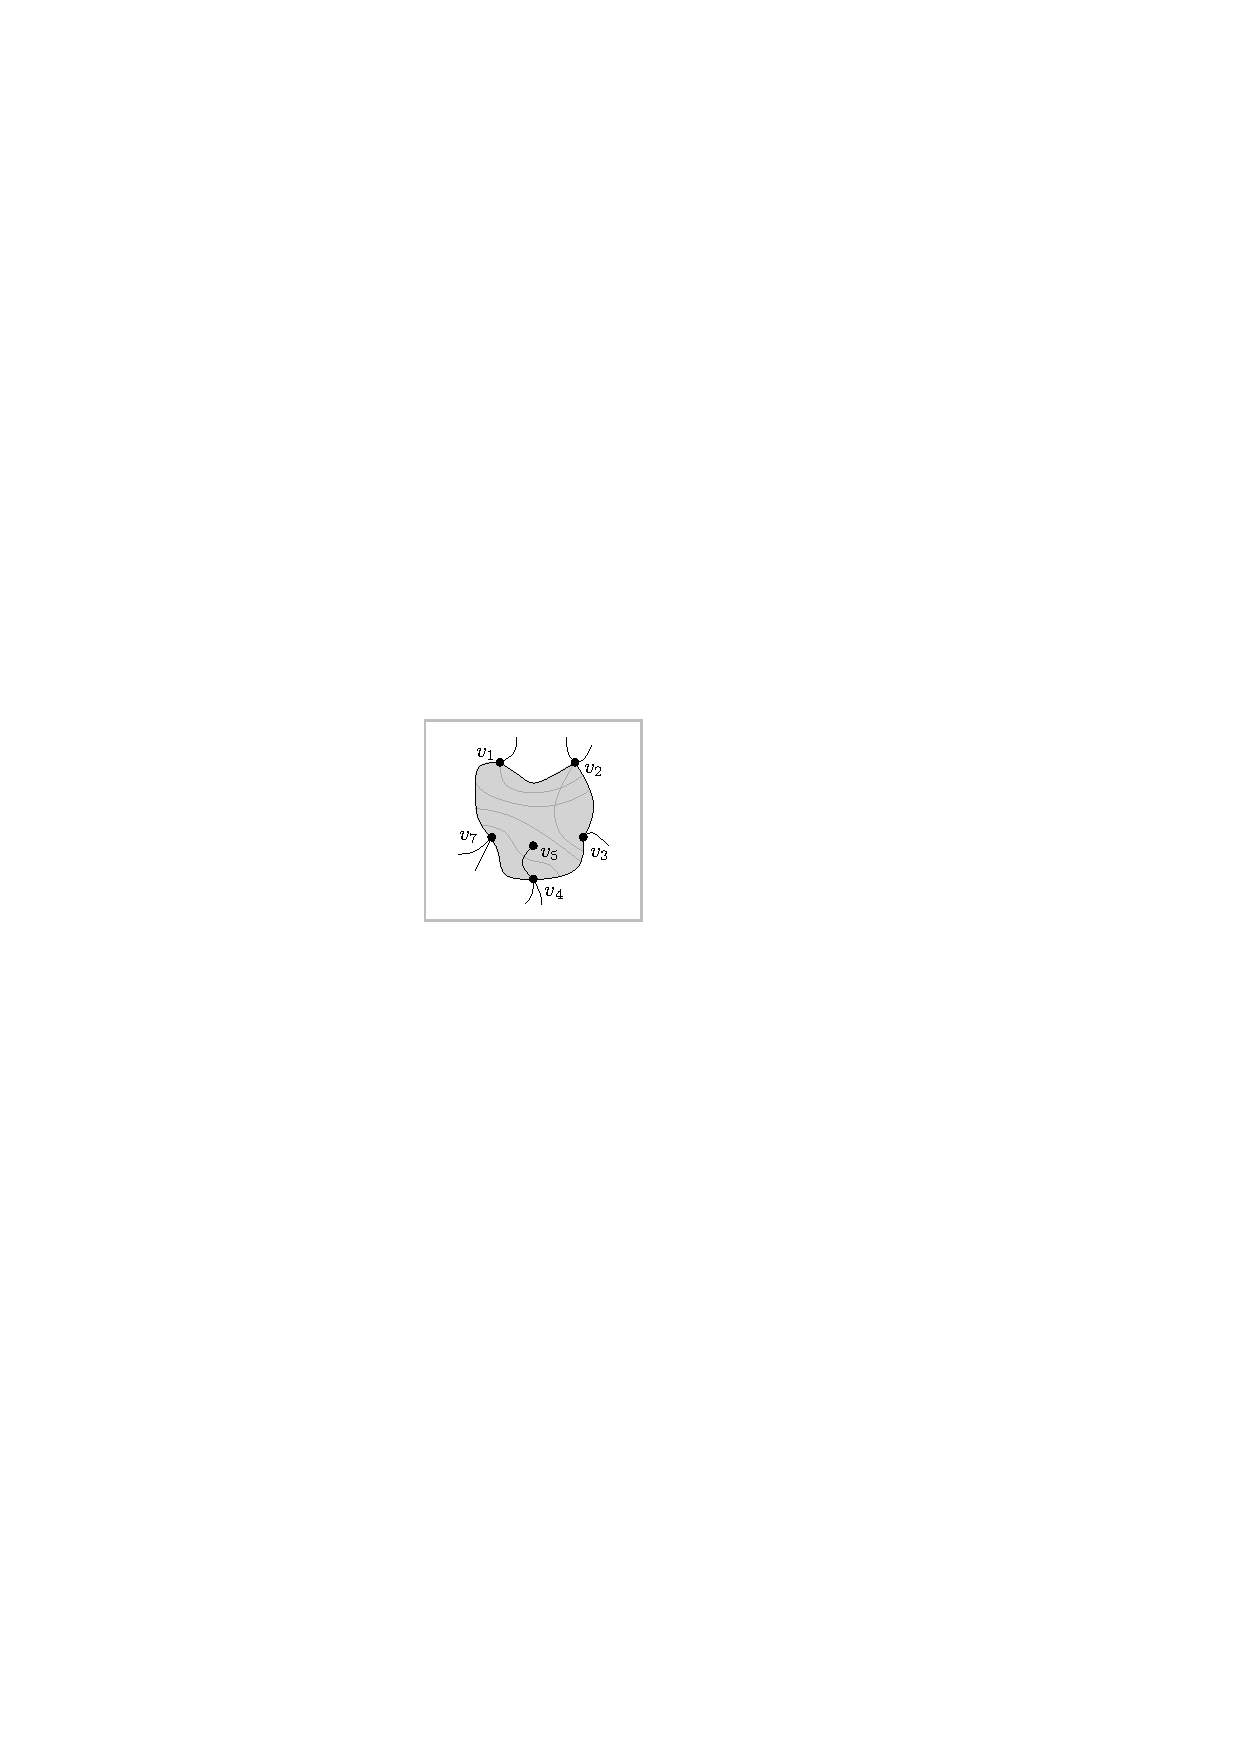
\includegraphics[width=\textwidth,page=1]{images/preliminaries}
        \subcaption{~}\label{fig:non_simple_face}
    \end{minipage}
	\begin{minipage}[b]{.18\textwidth}
        \centering
        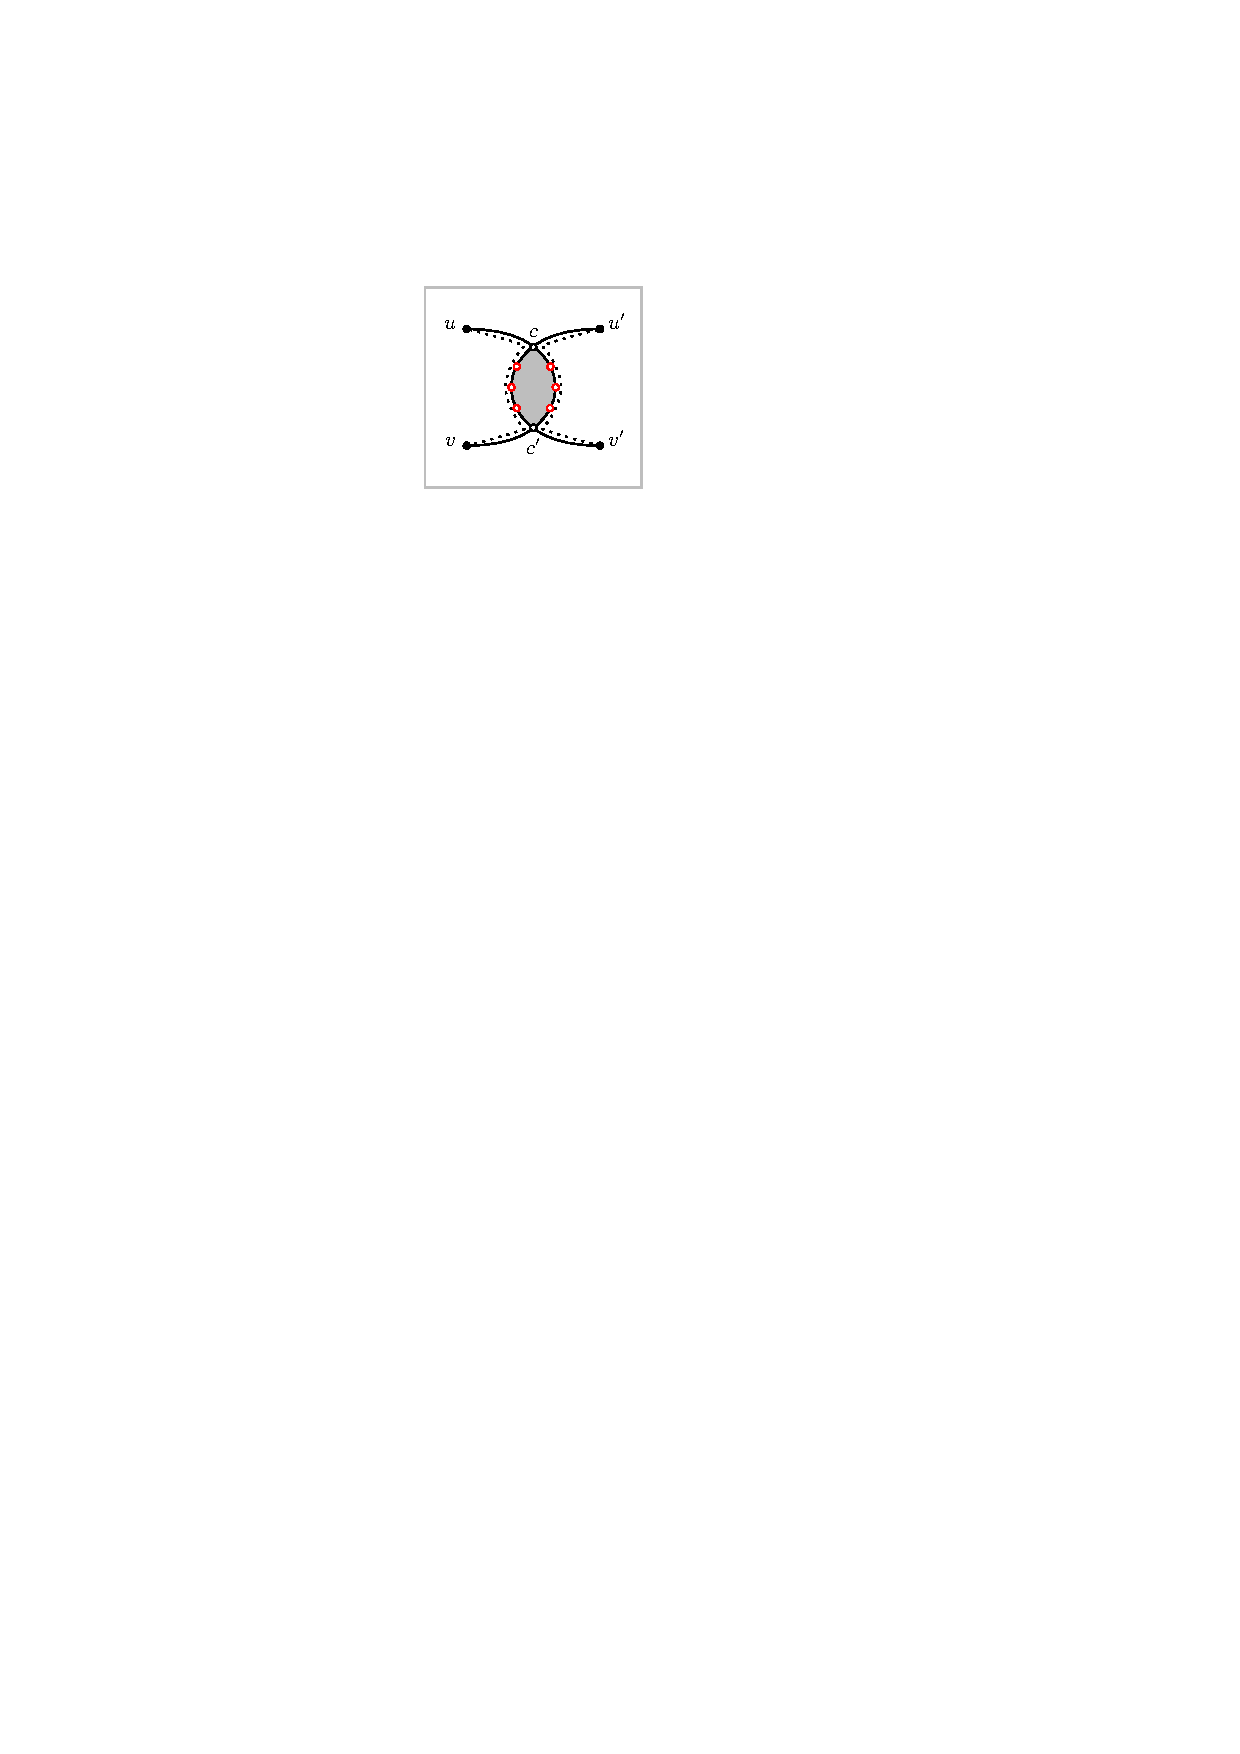
\includegraphics[width=\textwidth,page=1]{images/crossing_conf}
        \subcaption{~}\label{fig:crossing_twice}
    \end{minipage}	
    \begin{minipage}[b]{.18\textwidth}
        \centering
        \includegraphics[width=\textwidth,page=2]{images/crossing_conf}
        \subcaption{~}\label{fig:crossing_twice_2}
    \end{minipage}
    \begin{minipage}[b]{.18\textwidth}
        \centering
        \includegraphics[width=\textwidth,page=3]{images/crossing_conf}
        \subcaption{~}\label{fig:crossing_adjacent}
    \end{minipage}	
    \begin{minipage}[b]{.18\textwidth}
        \centering
        \includegraphics[width=\textwidth,page=4]{images/crossing_conf}
        \subcaption{~}\label{fig:crossing_adjacent_2}
    \end{minipage}	
    \caption{%
    (a)~A non-simple face $\{v_1,\ldots,v_7\}$, where $v_6$ is identified with $v_4$.
    Different configurations used in 
    (b-c)~Lemma~\ref{lem:crossing_twice}, and 
    (d-e)~Lemma~\ref{lem:crossing_adjacent}.}
    \label{fig:2_planar_polygon_conf}
\end{figure} 

Drawing $\Gamma(G)$ is called \emph{$k$-planar} if every edge in $\Gamma(G)$ is crossed at most $k$ times. Accordingly, a graph is called \emph{$k$-planar} if it admits a $k$-planar drawing. An \emph{optimal $k$-planar} graph is a $k$-planar graph with the maximum number of edges (e.g., an optimal $1$-planar graph on $n$ vertices is a $1$-planar graph with exactly $4n-8$ edges). For an optinal $k$-planar graph $G$ on $n$ vertices, a $k$-planar drawing $\Gamma(G)$ of $G$ is called \emph{planar-maximal crossing-minimal} or simply PMCM-drawing if and only if $\Gamma(G)$ has the maximum number of true-planar edges among all $k$-planar drawings of $G$ and, subject to this restriction, $\Gamma(G)$ has also the minimum number of crossings.

\begin{lemma}
Let $\Gamma(G)$ be a PMCM-drawing of an optimal $k$-planar graph $G$ in which two edges $(u,v)$ and $(u',v')$ cross more that once. Let $c$ and $c'$ be two consecutive crossing points of them. Then, the closed region $R_{c,c'}$ that is defined by $(u,v)$, $(u',v')$ and the crossing points $c$ and $c'$ has at least one vertex in its interior.
\label{lem:crossing_twice}
\end{lemma}
\begin{proof}
For a proof by contradiction, assume that there is no vertex in $R_{c,c'}$. Denote by $nc(u,v)$ and $nc(u',v')$ the number of crossings along $(u,v)$ and $(u',v')$ that are between $c$ and $c'$, respectively (red drawn in Figure~\ref{fig:crossing_twice}). First assume that $nc(u,v) = nc(u',v')$. We will cope with the case where $nc(u,v) \neq nc(u',v')$ shortly. We proceed by redrawing edge $(u,v)$ and $(u',v')$ so to eliminate both crossings $c$ and $c'$ without affecting the $k$-planarity of $G$; see the dotted-drawn edges of Figure~\ref{fig:crossing_twice}. Of course, this contradicts the crossing minimality of $\Gamma(G)$. To complete the proof of this lemma, it remains to consider the case where $nc(u,v) \neq nc(u',v')$. Assume w.l.o.g.~that $nc(u,v) > nc(u',v')$. In this case, there is at least one other edge, say $(u'',v'')$, that crosses $(u,v)$ between $c$ and $c'$ at least twice, say at points $d$ and $d'$; refer to Figure~\ref{fig:crossing_twice_2}. Since the ``length'' between $d$ and $d'$ is shorter than the length between $c$ and $c'$, it follows that if we apply the analysis above on $(u,v)$ and $(u'',v'')$, then there will be eventually a pair of crossing edges, say $e$ and $e'$, that will have exactly the same number of crossings, that is, $nc(e) = nc(e')$. This pair of edges contradicts the crossing minimality of $\Gamma(G)$.    
\end{proof}
 

\begin{lemma}
Let $\Gamma(G)$ be a PMCM-drawing of an optimal $k$-planar graph $G$ in which two edges $(u,v)$ and $(u,v')$ incident to a common vertex $u$ cross. Let $c$ be the first crossing point of $(u,v)$ with $(u,v')$ starting from $u$. Then, the closed region $R_{c}$ that is defined by vertex $u$, edges $(u,v)$, $(u,v')$ and $c$ has at least one vertex in its interior.
\label{lem:crossing_adjacent}
\end{lemma}
\begin{proof}
For a proof by contradiction, assume that there is no vertex in $R_{c}$. Denote by $nc(u,v)$ and $nc(u,v')$ the number of crossings along $(u,v)$ and $(u,v')$ that are between $u$ and $c$, respectively (red drawn in Figure~\ref{fig:crossing_twice_2}). First assume that $nc(u,v) = nc(u,v')$. We will cope with the case where $nc(u,v) \neq nc(u,v')$ shortly. We proceed by eliminating crossing $c$ without affecting the $k$-planarity of $G$; see the dotted-drawn edges of Figure~\ref{fig:crossing_adjacent}. Of course, this contradicts the crossing minimality of $\Gamma(G)$. To complete the proof of this property, it remains to consider the case where $nc(u,v) \neq nc(u,v')$. Assume w.l.o.g.~that $nc(u,v) > nc(u,v')$. In this case, there is either one other edge of $u$, say $(u,v'')$ that crosses $(u,v)$ between $u$ and $c$, or there exists an edge $(u'',v'')$ that crosses at least twice edge $(u,v)$. By Lemma~\ref{lem:crossing_twice}, the latter case would imply that $R_{c}$ is not an empty region; a contradiction. Hence, there exists at least one other edge, say $(u,v'')$, that crosses $(u,v)$ between $u$ and $c$, say at point $d$; refer to Figure~\ref{fig:crossing_adjacent_2}. Since the ``length'' between $u$ and $d$ is shorter than the length between $u$ and $c$, it follows that if we apply the analysis above on $(u,v)$ and $(u,v'')$, then there will be eventually a pair of crossing edges incident to $u$, say $e$ and $e'$ that have exactly the same number of crossings, that is, $nc(e) = nc(e')$. This pair of edges contradicts the crossing minimality of $\Gamma(G)$.   
\end{proof}

A Jordan curve $[u,v]$ joining vertices $u$ and $v$ of $G$ is a \emph{\pe} in drawing $\Gamma(G)$ if and only if $[u,v]$ is not a homotopic self-loop in $\Gamma(G)$, that is, either $u \neq v$ or $u=v$ and there is at least one vertex in the interior and the exterior of $[u,v]$. Note that $u$ and $v$ are not necessarily adjacent in $G$. However, since each topological edge $(u,v) \in E$ of $G$ is represented by a Jordan curve in $\Gamma(G)$, it follows that $(u,v)$ is by definition a \pe of $G$ (among other ones that can potentially exist).

We say that vertices $v_1,v_2,\dots,v_k$ define a \emph{\pp} in $\Gamma(G)$, if there exist \pes $[v_i,v_{i+1}]$, for $i=1,\dots, k-1$ and \pe $[v_1,v_k]$ of $\Gamma(G)$, which%
\begin{inparaenum}[(i)]
\item do not cross with each other and
\item define a region in $\Gamma(G)$ that has no vertices in its interior.
\end{inparaenum}
%
%We refer to the (empty of vertices) interior region of a \pp as a \emph{polygonal region} (denoted by $\mathcal{R}_k$), and to its boundary as a \emph{polygonal boundary} (denoted by $\mathcal{B}_k$).

Now, consider a pair of vertices $u$ and $v$ of $G$ that are not necessarily distinct. We say that $u$ and $v$ form a \emph{corner pair} if and only if an edge $(u,u')$ incident to $u$ crosses an edge $(v,v')$ incident to $v$ in $\Gamma(G)$; see Figure~\ref{fig:corner_pair}. Let $c$ be the crossing point of $(u,u')$ and $(v,v')$. Clearly, any Jordan curve $[u,v]$ joining vertices $u$ and $v$ defines a closed region $R_{u,v}$ with edge-segments $(u,c)$ and $(v,c)$. We call $[u,v]$ \emph{corner edge} w.r.t.~$(u,u')$ and $(v,v')$ if and only if $R_{u,v}$ has no vertices of $G$ in its interior.   

\begin{property}
In a PMCM-drawing $\Gamma(G)$ of an optimal $k$-planar graph $G$ any corner edge $[u,v]$ is a potential edge.
\label{prp:corner}
\end{property}
\begin{proof}
By the definition of potential edges, it follows that the property holds when $u \neq v$. Consider now the case where $u=v$. In this case $[u,v]$ is a self-loop; see Figure~\ref{fig:corner_pair_same}. If the property does not hold, then it follows that $[u,v]$ is a self-loop with no vertices either in its interior or in its exterior. The former case clearly contradicts Lemma~\ref{lem:crossing_adjacent}. So we may assume w.l.o.g.~that there is no vertex in the exterior of $[u,v]$; see Figure~\ref{fig:corner_pair_ext}. In this case, however, it follows that the two edges $(u,u')$ and $(v,v')$ defining $[u,v]$ must cross more than once in the exterior of $[u,v]$, which leads to a contradiction with Lemma~\ref{lem:crossing_adjacent}.
\end{proof}

 \begin{figure}[tb]
    \centering		
    \begin{minipage}[b]{.16\textwidth}
        \centering
        \includegraphics[width=\textwidth,page=2]{images/preliminaries}
        \subcaption{~}\label{fig:corner_pair}
    \end{minipage}
    \begin{minipage}[b]{.16\textwidth}
        \centering
        \includegraphics[width=\textwidth,page=3]{images/preliminaries}
        \subcaption{~}\label{fig:corner_pair_same}
    \end{minipage}
    \begin{minipage}[b]{.16\textwidth}
        \centering
        \includegraphics[width=\textwidth,page=4]{images/preliminaries}
        \subcaption{~}\label{fig:corner_pair_ext}
    \end{minipage}
    \begin{minipage}[b]{.16\textwidth}
        \centering
        \includegraphics[width=\textwidth,page=5]{images/preliminaries}
        \subcaption{~}\label{fig:parallel_pair}
    \end{minipage}
	\begin{minipage}[b]{.16\textwidth}
        \centering
        \includegraphics[width=\textwidth,page=6]{images/preliminaries}
        \subcaption{~}\label{fig:parallel_pair_same}
    \end{minipage}
	\begin{minipage}[b]{.16\textwidth}
        \centering
        \includegraphics[width=\textwidth,page=7]{images/preliminaries}
        \subcaption{~}\label{fig:parallel_pair_homotopic}
    \end{minipage}
    \caption{%    
    (a-c)~vertices $u$ and $v$ form a corner pair;
    (d-e)~vertices $u$ and $v$ form a parallel pair; 
    (f)~at least one of the two potential parallel edges exists.}
    \label{fig:crossing_confs}
\end{figure} 

We say that vertices $u$ and $v$ form a \emph{parallel pair} if and only if an edge $(u,u')$ of $u$ and an edge $(v,v')$ of $v$ both cross a third edge $(w,w')$ in $\Gamma(G)$ and additionally $(u,u')$ is not identified with $(v,v')$; see Figure~\ref{fig:parallel_pair}. Let $c$ and $c'$ be the crossing points of $(u,u')$ and $(v,v')$ with $(w,w')$, respectively. Clearly, any Jordan curve $[u,v]$ joining vertices $u$ and $v$ defines a closed region $R_{u,v}$ with edge-segments $(u,c)$, $(c,c')$ and $(v,c')$. We call $[u,v]$ \emph{parallel edge} w.r.t.~$(u,u')$ and $(v,v')$ if and only if $R_{u,v}$ has no vertices of $G$ in its interior. Symmetrically we define region $R_{u',v'}$ and parallel edge $[u',v']$ w.r.t.~$(u,u')$ and $(v,v')$.

%We denote a corner (parallel) pair formed by $u$ and $v$ by $\ppp{u}{v}$ ($\ppc{u}{v}$, resp.). We have the following properties:

\begin{property}
In a PMCM-drawing $\Gamma(G)$ of an optimal $k$-planar graph $G$ at least one of parallel edges $[u,v]$, $[u',v']$ is a potential edge.
\label{prp:parallel}
\end{property}
\begin{proof}
For a proof by contradiction, assume that neither $[u,v]$ nor $[u',v']$ is a potential edge. This implies that $u=v$, $u'=v'$ and both $[u,v]$ and $[u',v']$ are self-loops that have no vertices in their interiors or their exteriors. Figure~\ref{fig:parallel_pair_homotopic} illustrates the case where both $[u,v]$ and $[u',v']$ are self-loops with no vertices in their interiors; the other cases are symmetric. It is not hard to see that $(u,u')$ and $(v,v')$ are homotopic parallel edges; a contradiction.
\end{proof}
%
We say that $(u,u')$ and $(v,v')$ are \emph{independent} if and only if both parallel edges $[u,v]$ and $[u',v']$ are \pes.

\begin{remark}
Note that in the definition of parallel pairs we required $(u,u')$ not to be identified with $(v,v')$. If this is not the case, then edge $(w,w')$ is being crossed twice by $(u,u') = (v,v')$. To make the description of our proofs simple, in Sections~\ref{sec:2planar} and \ref{sec:3planar} we will initially require that every pair of edges in $\Gamma(G)$ crosses at most once. We will call a drawing fulfilling this requirement \emph{almost-simple}. This requirement will be formally proved in both cases (see Lemmas~\ref{lem:2_planar_cross_twice} and~\ref{lem:3_planar_cross_twice}).    
\end{remark}



